\documentclass[10pt, usenames, dvipsnames, table]{beamer}
\usetheme{Berkeley}
\usecolortheme{seagull}
\usepackage{graphicx}
\graphicspath{ {../images/} }
\usepackage{array}
\RequirePackage{fix-cm}
\usepackage{colortbl}
\usepackage{hyperref}
\usepackage{graphbox}
\usepackage{algorithm}
\usepackage{algpseudocode}
\usepackage{minted}
\setminted{} % numbers=right, bgcolor=lightgray}


\title{The Scala Programming Language}
\author{Troy Hut and Benjamin Killeen}
\date{}

\begin{document}

\begin{frame}
  \titlepage{}
\end{frame}

\section{Introduction}
\begin{frame}
  \frametitle{Introduction}
  Scala is:
  \begin{itemize}
  \item<2-> Object oriented
  \item<3-> Functional
  \item<4-> Statically typed
  \end{itemize}
\end{frame}

\begin{frame}
  \frametitle{Scala is \textbf{Scalable}}
  \begin{figure}
    \centering
    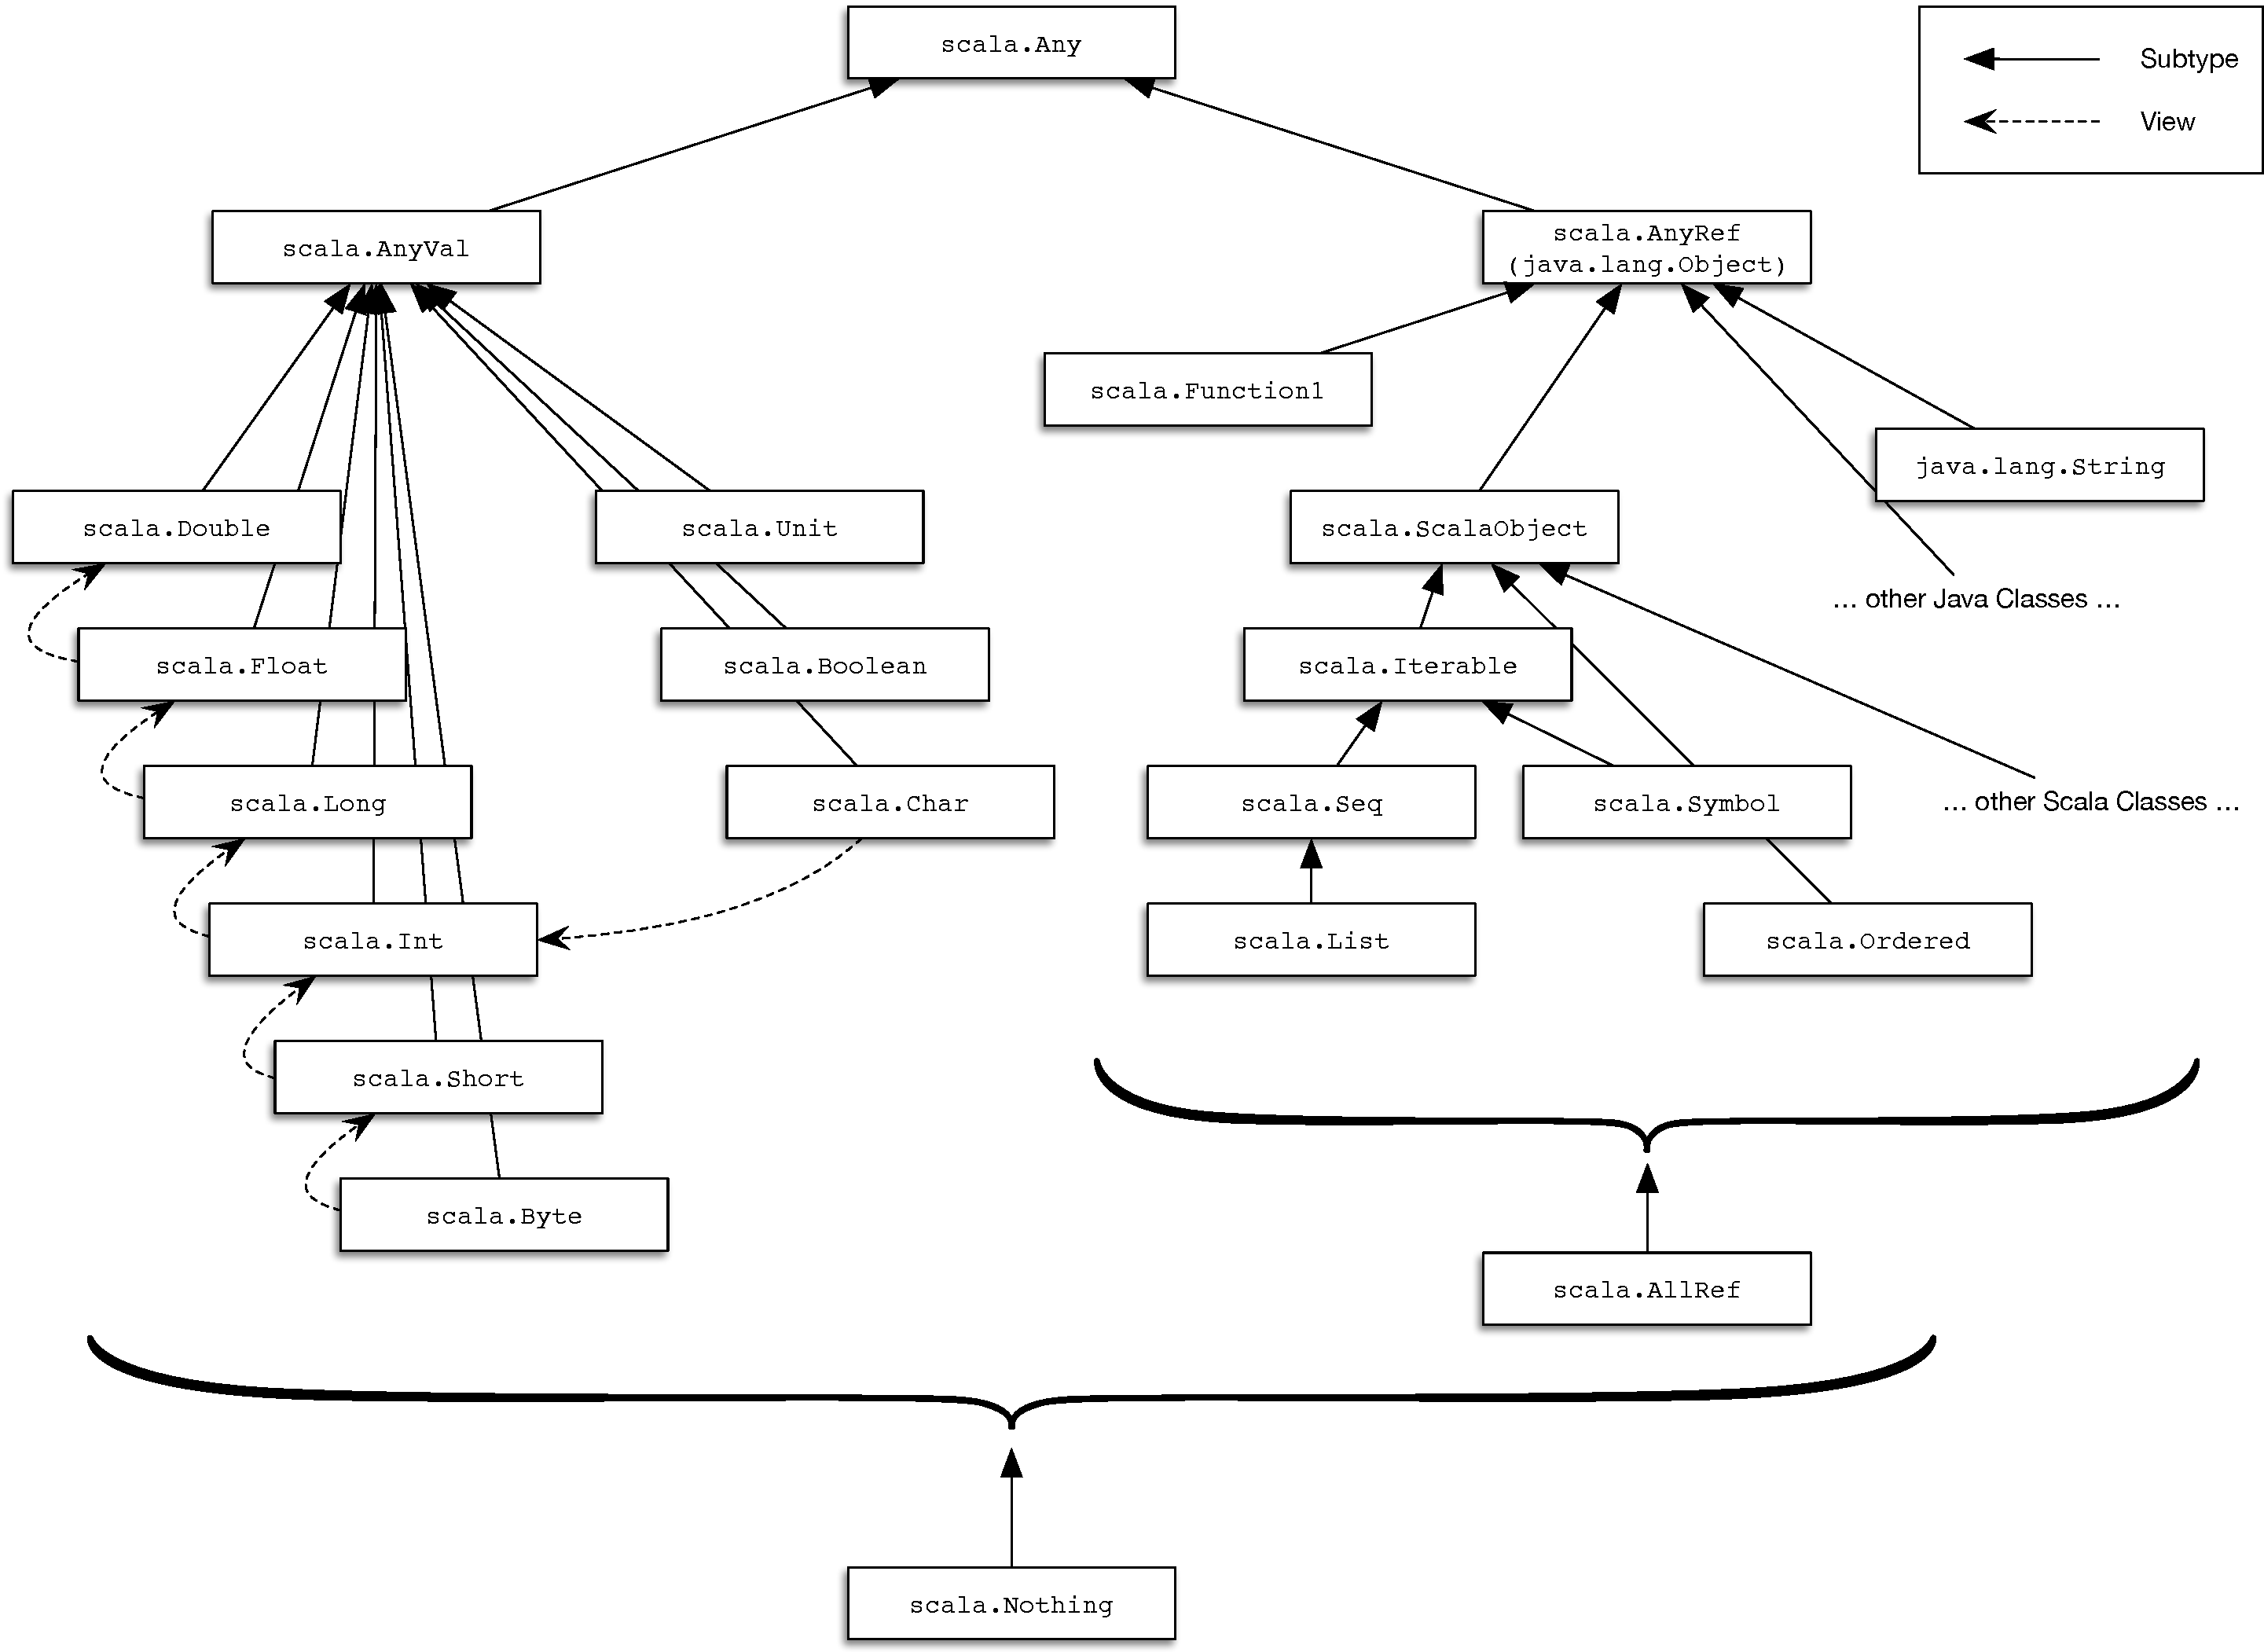
\includegraphics[width=0.8\linewidth]{scala_classes}
    \caption{The Scala class hierarchy.}
    \label{fig:class_hierarchy}
  \end{figure}
\end{frame}

\begin{frame}
  \frametitle{Naturals}
  \begin{listing}
    \inputminted{Scala}{../examples/nats.scala}
    \caption{An implementation of naturals.}
    \label{lst:nats-example}
  \end{listing}
  
\end{frame}

\end{document}
%%% Local Variables:
%%% mode: latex
%%% TeX-master: t
%%% TeX-command-extra-options: "-shell-escape"
%%% End:
